\section{Abbildungen: $\mathbb{R}^n \rightarrow \mathbb{R}$}

\subsection{Linearisierung}
\begin{equation*}
	f(x_1 + \Delta x_1, x_2 + \Delta x_2, \cdots x_n + \Delta x_n) \approx f(x_1 \cdots x_n) + \frac{\delta f}{\delta x_1} \cdot \Delta x_1 \cdots + \frac{\delta f}{\delta x_n} \cdot \Delta x_n
\end{equation*}

\subsection{Fehlerrechnung}
\begin{equation*}
	e_{max} = \bigg | \frac{\delta f}{\delta x_1}(\bar{x_1} \cdots \bar{x_n}) \cdot \Delta x_1 \bigg | + \cdots + \bigg | \frac{\delta f}{\delta x_n}(\bar{x_1} \cdots \bar{x_n}) \cdot \Delta x_n \bigg |
\end{equation*}
($\Delta x_i$ ist die Messabweichung, $\bar{x_i}$ der Messwert)

\subsection{Richtungsableitung}
\begin{itemize}
	\item Gradient:
		$G_f = \big(\frac{\delta f}{\delta x_1}, \frac{\delta f}{\delta x_2}, \cdots \frac{\delta f}{\delta x_n}\big )$
	\item Richtungsableitung:
		$f'_v(x_1, x_2, \cdots x_n) = \vec{v} \cdot G_f	$
	\item Steigungsgerade:
		$g(x_1, x_2, \cdots x_n) = P + \lambda G_f(P)$

		\begin{itemize}
			\item Richtung maximaler Steigung an einem Punkt P \\
			$\vec{d} = G_f(P)$
			\item Steigung in Richtung $\vec{d}$ \\ $m = |\vec{d}|$
			\item Steigungswinkel \\ $\alpha = arctan(m)$
		\end{itemize}
\end{itemize}

\subsection{Integration}
\begin{itemize}
	\item Doppelintegral (Funktionen mit mehreren Parametern) \\
	$\int_B h(x, y) = \int_{a1}^{a2}(\int_{b1}^{b2} h(x, y) dy) dx$
    \begin{figure}[h!]
        \centering
        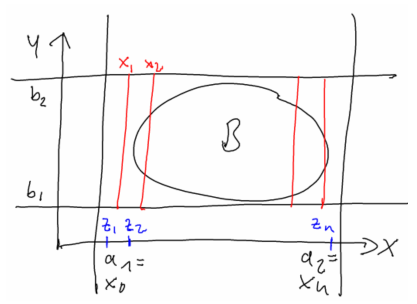
\includegraphics[scale=.5]{pics/doppelintegral}
        \caption{Integral über Abschnitte a und b}
    \end{figure}

	\item Geschachtelte Funktionen \\
	$\int_{B_{\arrowvert_{f(x)}^{g(x)}}} h(x, y) = \int_{a1}^{a2}(\int_{f(x)}^{g(x)} h(x, y) dy) dx$
    \begin{figure}[h!]
        \centering
        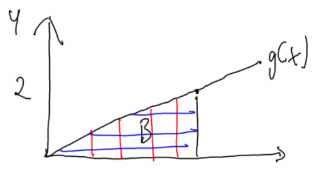
\includegraphics[scale=.5]{pics/doppelintegralfunktionen}
        \caption{Integral über Abschnitte a und (g - f)}
    \end{figure}

	\item Allgemein gilt: \\
	Sind $f_{x,y}$ und $f_{y,x}$ stetig, so ist $f_{x,y} = f_{y,x}$
\end{itemize}

\subsection{Extremwerte}
\subsubsection{Rezept: Minimum/Maximum}
\begin{enumerate}
	\item $\frac{\delta}{\delta x}f(x_0,y_0) = 0 \wedge \frac{\delta}{\delta y}f(x_0,y_0) = 0$ Extremwert

	\item $\Delta = \frac{\delta \delta}{\delta \delta x}f(x_0,y_0) \cdot \frac{\delta \delta}{\delta \delta y}f(y_0,y_0) \cdot (\frac{\delta}{\delta x \delta y}f(x_0,x_0))^2$
	\begin{itemize}
		\item $\frac{\delta \delta}{\delta \delta x}f(x_0,y_0) < 0$ relatives Maximum
		\item $\frac{\delta \delta}{\delta \delta x}f(x_0,y_0) > 0$ relatives Minimum
		\item $\Delta < 0$ Sattelpunkt
		\item $\Delta = 0$ nicht Entscheidbar
	\end{itemize}
\end{enumerate}
